\chapter{ISTTOK control implementations and results }

Using the multi-filament centroid position reconstruction currently available in real-time for all the discharges, is possible to foray into control techniques and its real-time implementation. This chapter describes the latest implementations in ISTTOK's  MARTe framework followed by the presentation of the obtained results for control of the vertical and radial current centroid position.

\section{Implementation of the General Application Modules }

As mentioned in previous sections, ISTTOK operates on top of the MARTe framework who in turn is basically constructed by a set of General Application Modules (GAM) as described in chapter 2. The control of the plasma current centroid position is achieved by means of several GAMs working altogether,  figure ~\ref{GAMsDiags} depicts a scheme of how the control loop works. It starts by acquiring  the signals from the magnetic probes and processing them in the "Magnetics" GAM where the radial and vertical centroid position are computed for every MARTe cycle. The "Controller" GAM selects the controller to be used for the centroid position based on the retrieved data from a GUI "Discharge Configurator" the tokamak operator has already configured before the discharge starts. Depending on the controller selection there is a "PID" GAM and a "LQR" GAM , based on the control algorithms studied in Chapter 2.4. After the "PID" GAM or the "LQR" GAM computed the required  inputs of the system these values are sent back to the "Controller" GAM which then sends them as command signals to the power supplies of the PF coils.\smallskip

\begin{figure}[h]
	\centering
	\includegraphics[width=1.0\textwidth]{Chp5/GAMsDiagram.png}	
	\caption{ISTTOK MARTe overall control position  scheme. \label{GAMsDiags}}
\end{figure}

Since ISTTOK is and AC tokamak during the transition from negative to positive, or opposite, plasma current there is no reconstruction of the centroid position, then a pre-programmed configuration of the  PF coils currents acts during this transition of $~\approx~1ms$, which means there is a constant switching from automatic to manual control in between plasma cycles, the switching process between controllers produces jumps at the plant inputs, this is known as the bumpless transfer problem ~\cite[Chapter~8]{Hippe2011}. To remove the jump, the controller output  should be made as close as possible to the output during manual mode. Then the jump at the instant of switching will be minimized~\cite{Vrancic1996}.   

\subsection{PID control implementation}

Early tokamaks used sets of poloidal field coils symmetrically placed with respect to the tokamak equatorial plane to guarantee mutually independent vertical and horizontal movement of the plasma~\cite[Chapter~1]{PirontiBook}.  For many years, ISTTOK control relied on the principle that due to Lorentz force law, the control strategy could simply be driven by the principle that an external vertical field  generates an horizontal force and a horizontal external field generates a vertical force, having thus two separate SISO controllers for the vertical and radial centroid position. The "PID" GAM is responsible for this function, it has two PID  controllers, concept deeply addressed in section ~\ref{PID_sec},   with pre-configuration gains, in addition they have a    anti-windup \footnote{The saturation of actuators or major set point changes are some  of the most frequent nonlinearities in control applications and they can cause instabilities in the system, the undesired effect of this events is called windup and typically it produces undesired overshoots resulting from overreaction in the integrator of a PID controller ~\cite[Chapter~1]{Hippe2011}.} action that basically consists in an adjustment of the integral action when the saturation limits are reached along with a correction of the bumpless transfer   just when the transition from manual to automatic control happens ~\cite[Chapter~3]{Yu2011}. \smallskip  

The PID equations are digitally implemented in the "PID" GAM as ~\cite[Chapter~1]{Yu2011}: 
\begin{equation}
	u[k]=K_p~e[k]+ K_i~T_s\sum_{i=1}^{k}e[i]+\frac{K_d}{T_s}(e[k]-e[k-1])
\end{equation}

where $u[k]$ is the controlled output signal, for ISTTOK it corresponds to the vertical and horizontal PF coils currents,$K_p,~K_d$ and $K_i$ are the PID gains and $e[k]$ is error variable which in this case is  the vertical or horizontal plasma centroid position minus a given set point programmed by the operator in the "Discharge configurator".

\subsection{Data-driven state-space model retrieving }

Data-driven dynamical systems is a rapidly evolving field, data are abundant, while physical laws or governing equations remain elusive even in classical fields, such as optics and turbulence, where governing equations do exist, researchers are increasingly turning toward data-driven analysis~\cite[Chapter~7]{DataDriven2019}.\smallskip

Early efforts in finding a theoretical model for ISTTOK magnetic control were performed during  the last years. Since ISTTOK PF coils are not axisymmetric a working theoretical model  was never successfully retrieved. This fact made necessary to find a novel form to implement a model-based magnetic control on ISTTOK real-time MARTe platform.   Through  the \textit{System Identification Toolbox} from \textsc{Matlab}, whose background concepts were explained in chapter~\ref{Disc_SS_ident}, state-space models were retrieved. This models have as inputs the PF vertical and horizontal currents and as outputs the vertical and radial plasma current centroid position, having thus  $2\times 2$ MIMO systems. During this process data from several discharges were used in order to obtained  sufficiently  accurate models. When joining data sets of signals from  positive and negative plasma current discharges  the models started to not be consistent showing since early stages that the tokamak needed to be modeled separately: one state-space model for discharges were $I_p > 0$ and another for discharges where $I_p>0$. This matter probably originates from the fact that a  tokamak is not completely axisymmetric in reality, and particularly for ISTTOK, it happens to have a very non-axisymmetric PF coils. Figure ~\ref{SimResp_pos} and figure ~\ref{SimResp_neg} show the comparison between  the data-base centroid position signal and its reconstruction using the estimated state-space models. These are validation plots , which means the signals from the reconstruction of the centroid position were not used as modeling data, differences in the transients of the signals might be originated fro the differences in initial states between systems.\smallskip



\begin{figure}
	\begin{subfigure}[b]{0.55\textwidth}
		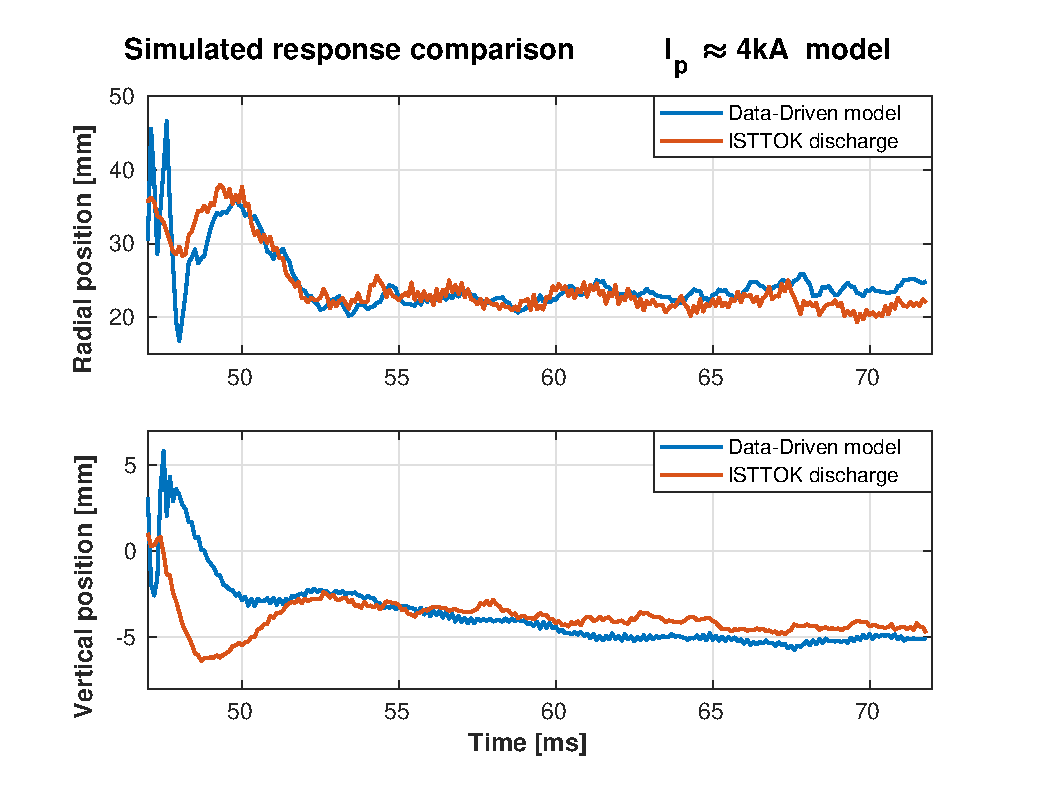
\includegraphics[width=\textwidth]{Chp5/SimResp_559.eps}  
		\caption{Comparison between the  identified model response and the real-time centroid position reconstruction. Shot $\#48559 $\label{SimResp559} }
	\end{subfigure}
	~ %add desired spacing between images, e. g. ~, \quad, \qquad, \hfill etc. 
	%(or a blank line to force the subfigure onto a new line)
	\begin{subfigure}[b]{0.55\textwidth}
		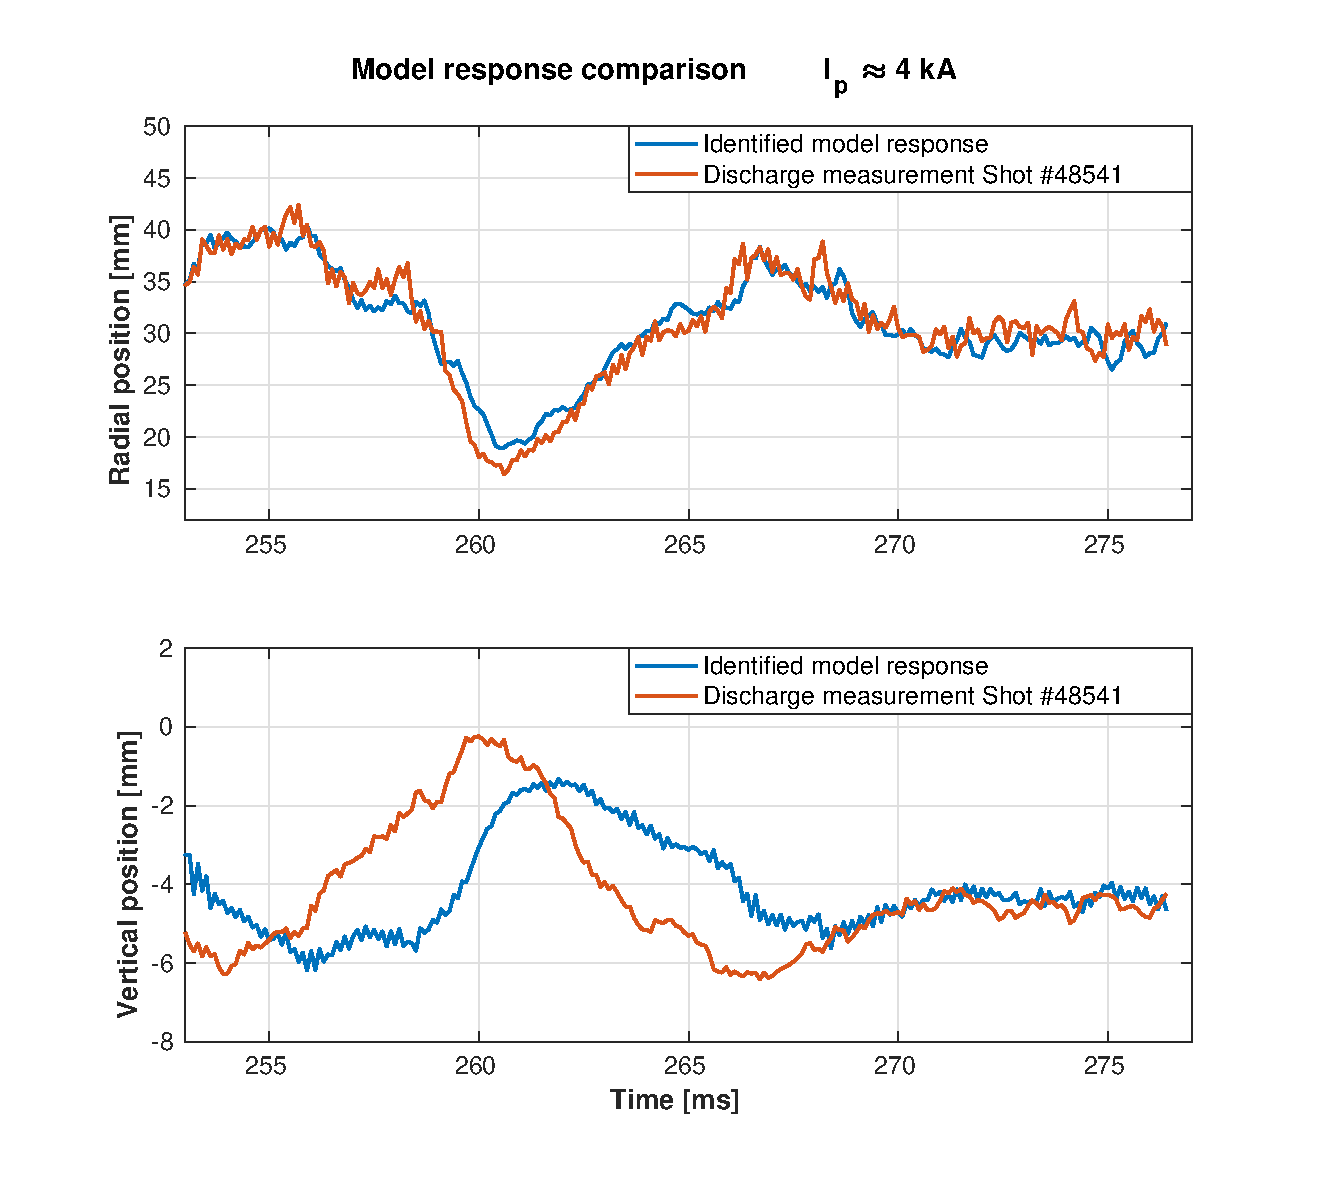
\includegraphics[width=\textwidth]{Chp5/SimResp_541.eps}        
		\caption{ Comparison between the  identified model response and the real-time centroid position reconstruction. Shot $\#48541 $ \label{SimResp541}}
	\end{subfigure}
	\caption{Model response for two different  $I_p~\approx 4~kA$ discharges. \label{SimResp_pos}}
\end{figure}


\begin{figure}
	\begin{subfigure}[b]{0.55\textwidth}
		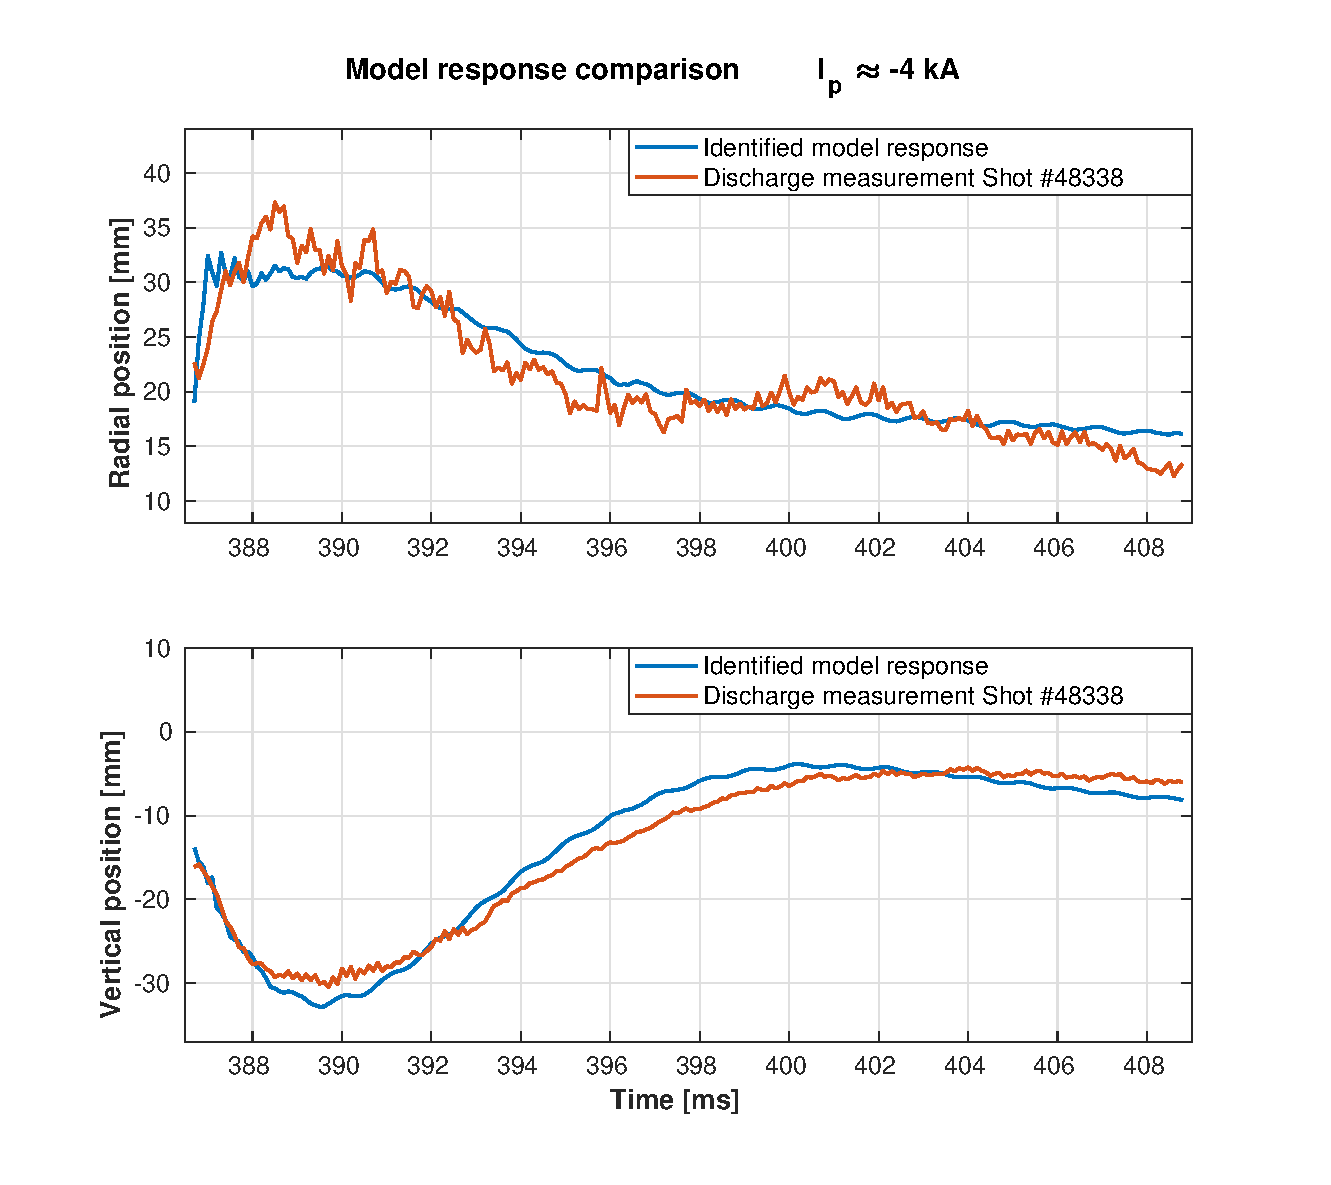
\includegraphics[width=\textwidth]{Chp5/SimResp_338.eps}  
		\caption{Comparison between the  identified model response and the real-time centroid position reconstruction. Shot $\#48338 $ \label{SimResp338} }
	\end{subfigure}
	~ %add desired spacing between images, e. g. ~, \quad, \qquad, \hfill etc. 
	%(or a blank line to force the subfigure onto a new line)
	\begin{subfigure}[b]{0.55\textwidth}
		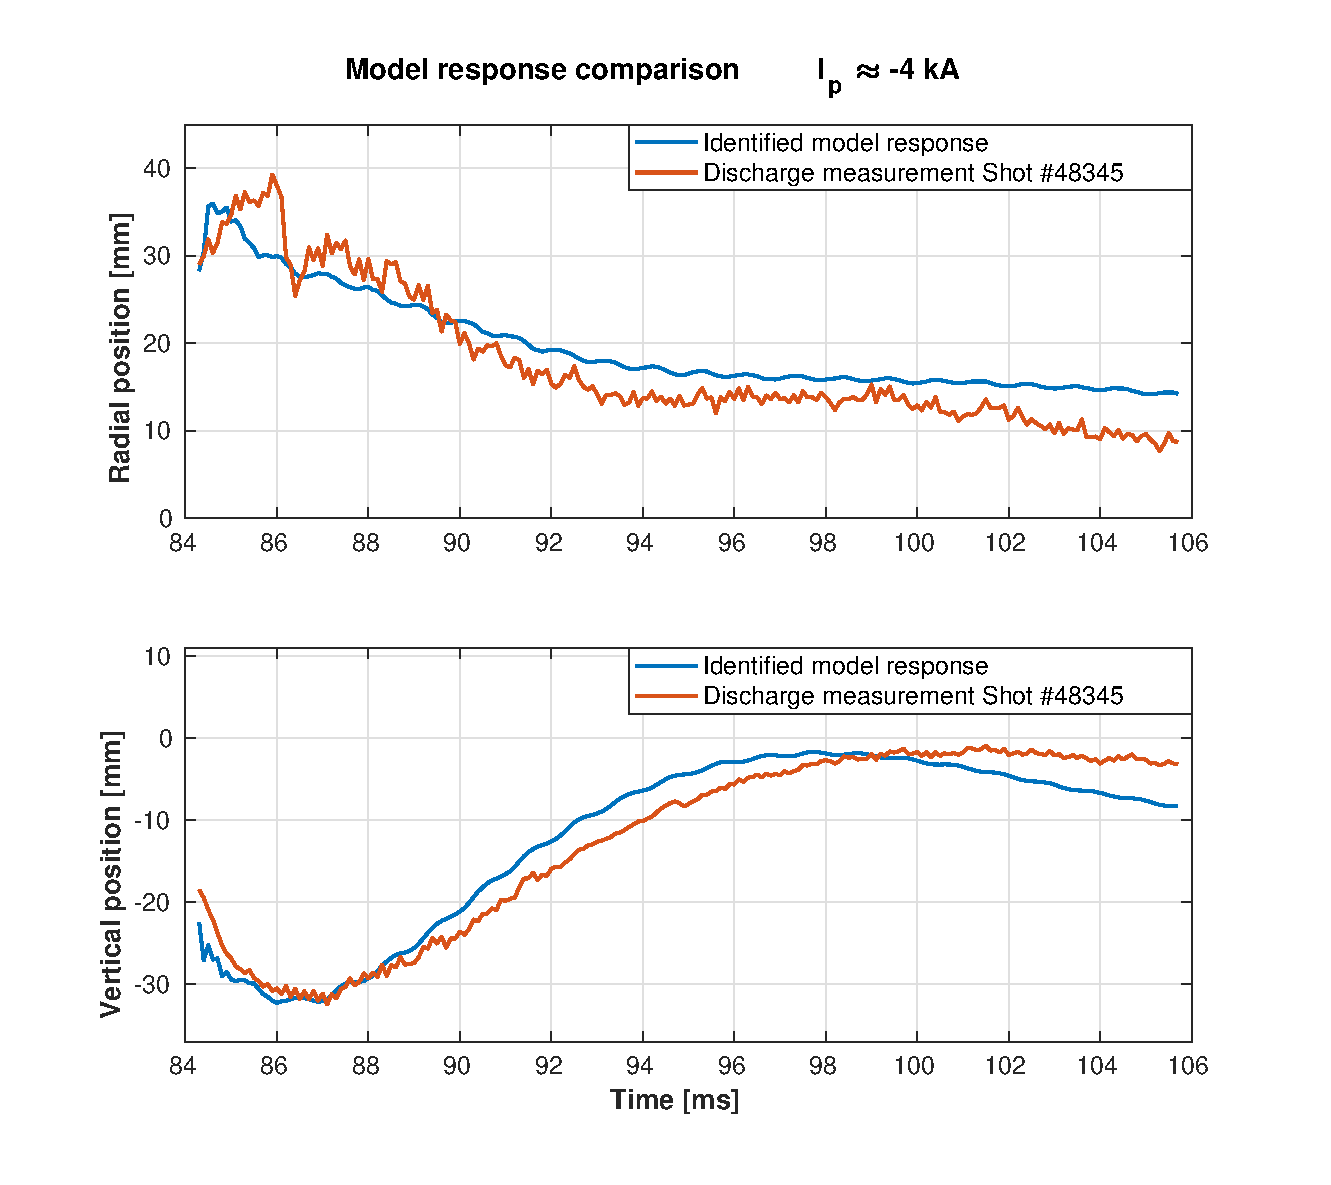
\includegraphics[width=\textwidth]{Chp5/SimResp_345.eps}        
		\caption{ Comparison between the  identified model response and the real-time centroid position reconstruction. Shot $\#48345 $ \label{SimResp345}}
	\end{subfigure}
	\caption{ Model response for two $I_p~\approx -4~kA$ discharges. \label{SimResp_neg}}
\end{figure}

Since a tokamak is not a linear system, the modeling process was done using data sets where the centroid position was located in a certain region of values in order to approximate the estimated  model to an equilibrium region where a linear model approximation is valid. The optimal number of states computationally retrieved was  10. 


\subsection{Kalman filter implementation}

After retrieving the state-space models for the plasma centroid position, the next goal is to implement a MIMO controller based on them. In order to reconstruct the states vector $x$ two Kalman filters ware implemented, one for plasma current positive model and another for the negative model. The Kalman filter matrices were obtained  based on noise vectors from ISTTOK real data calculating  the covariance matrices from the signal vectors ~\cite{Mele2018}.  Figure ~\ref{Kalman_neg} and~\ref{Kalman_pos} correspond to the real-time Kalman filter reconstruction of the vertical and radial plasma centroid position and its comparison with the multi-filament reconstructed  position computed at the "Magnetics" GAM.\smallskip

\begin{figure}[h]
	\centering
	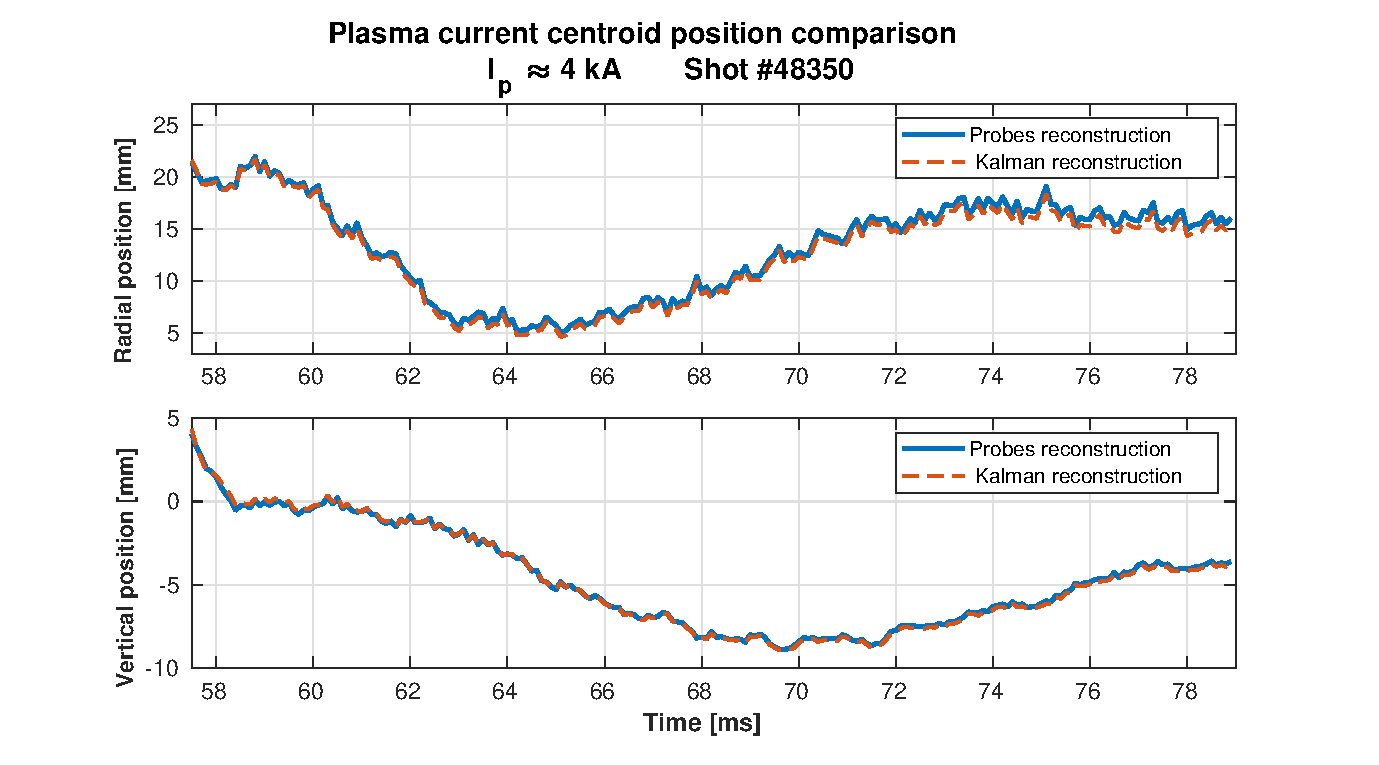
\includegraphics[width=0.85\textwidth]{Chp5/Kalman_comp_pos.eps}
	\caption{ Comparison of the real-time Kalman filter retrieved centroid position and the multi-filament reconstruction time trace for $I_p>0$.\label{Kalman_pos}}
\end{figure}

\begin{figure}[h]
	\centering
	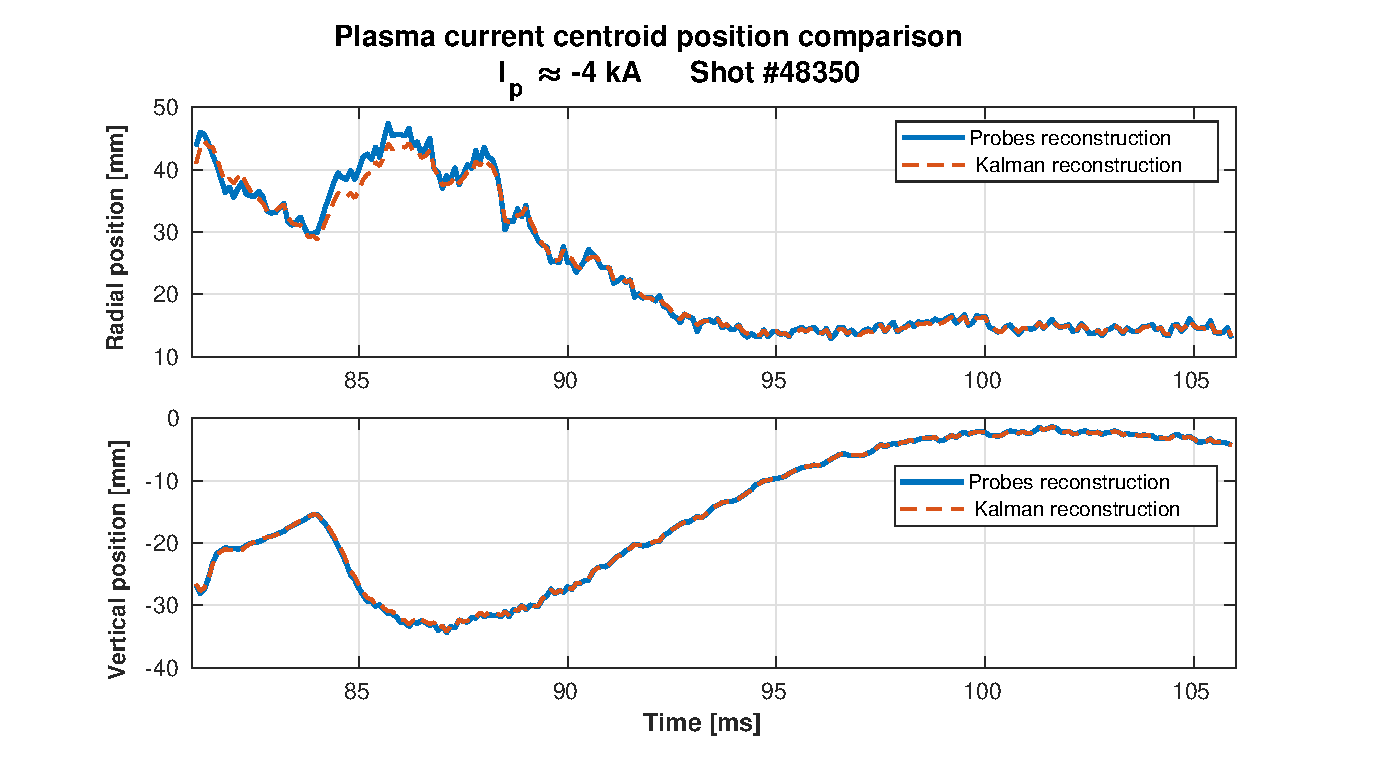
\includegraphics[width=0.85\textwidth]{Chp5/Kalman_comp_neg.eps}
	\caption{ Comparison of the real-time Kalman filter retrieved centroid position and the multi-filament reconstruction time trace for $I_p<0$\label{Kalman_neg}}
\end{figure}

\subsection{Multiple-Input Multiple-Output control implementation}



The full-state estimate from the Kalman filter is generally used in conjunction with the
full-state feedback control law from LQR, resulting in optimal sensor-based feedback. Combining the LQR full-state feedback with the Kalman fitler full-state estimator results in the linear-quadratic Gaussian (LQG) controller ~\cite[Chapter~8]{DataDriven2019}. Under this principle the real-time reconstructed states are multiplied by the control LQR gain $K$ in order to take the the vertical and radial plasma centroid position to a certain set point, this process is computed in the "LQR" GAM. The weight matrices for the LQR controller were empirical tuned in order to have a balance between a fast response and a not so energetically demanding input, several algorithms for a non-empirical calculation of the LQR matrices exist some of them propose a tuning based on experimental data with a gain matrix that can be iterative updated ~\cite[Chapter~9]{Franklin1998}, ~\cite{Trimpe2014}.
\smallskip



\subsubsection{Pole-zeros map}



Given the transfer function $H(s)\frac{b(s)}{a(s)}$ the value of $s$ such that $b(s)=0$ are places where $H(s)$ is zero, and the corresponding $s$ locations are called zeros. The  concept of pole  was introduced in section ~\ref{MIMO_sec}.  A Pole-zeros map is a representation in the complex plain n of the poles and zeros location of a system, either is in open-loop or in closed-loop. Since the data-driven models and its controllers are discrete the pole stability is given in a different form as in the continues time case,  figure~\ref{PoleZeroMap} shows the stable location of discrete poles($|\lambda|=1$),  the locations of the zeros have no role in determining the system stability.\smallskip



\begin{figure}[h]
	\centering
	\includegraphics[width=0.7\textwidth]{Chp5/PolesZerosMaps.png}
	
	\caption{ The matrix exponential defines a conformal map on the complex plane, mapping stable eigenvalues in the left half plane for continuous systems into eigenvalues inside the unit circle for discrete ~\cite[Chapter~8]{DataDriven2019}\label{PoleZeroMap}.}
\end{figure}

Figures \ref{PoleZeroClosePos} and ~\ref{PoleZeroClosePosZoom} correspond to the pole-zero maps for the state-space model where $I_p\approx 4~kA$ in closed loop and figures ~\ref{PoleZeroOpenPos} and ~\ref{PoleZeroOpenPosZoom} to the same system in open-loop. Figures ~\ref{PoleZeroCloseNeg} and ~\ref{PoleZeroCloseNegZoom} correspond to the pole-zero maps for the state-space model where $I_p\approx -4~kA$ and figures ~\ref{PoleZeroOpenNeg} and ~\ref{PoleZeroOpenNegZoom} to the same system in open-loop. It should be noticed that since the data-driven models are $2\times2$ MIMO systems each case is formed by 4 pole-zero maps.\smallskip
 


%% Positives
\begin{figure}
	\centering
	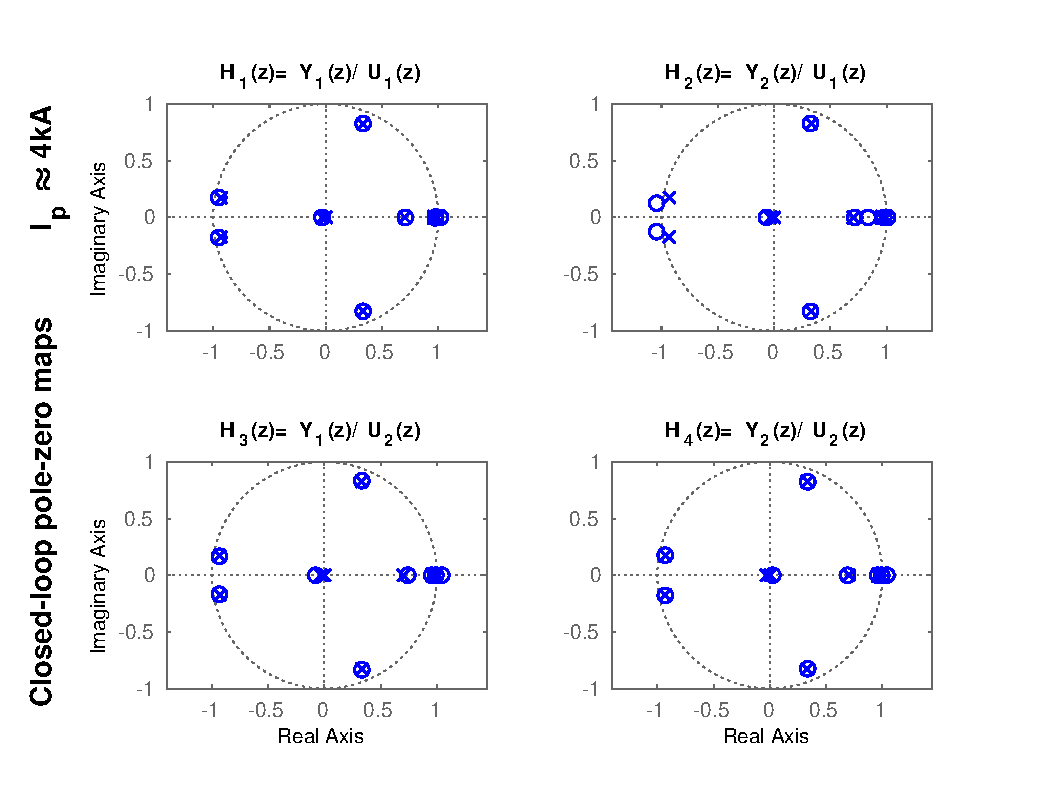
\includegraphics[width=0.85\textwidth]{Chp5/PoleZero/PoleZeroClosePos.eps}
	\caption{Pole-zero maps in closed loop for the model when $I_p\approx 4 kA$. Superposition  of poles and zeros can be seen in the four transfer functions.\label{PoleZeroClosePos}}
\end{figure}	

\begin{figure}
	\centering
	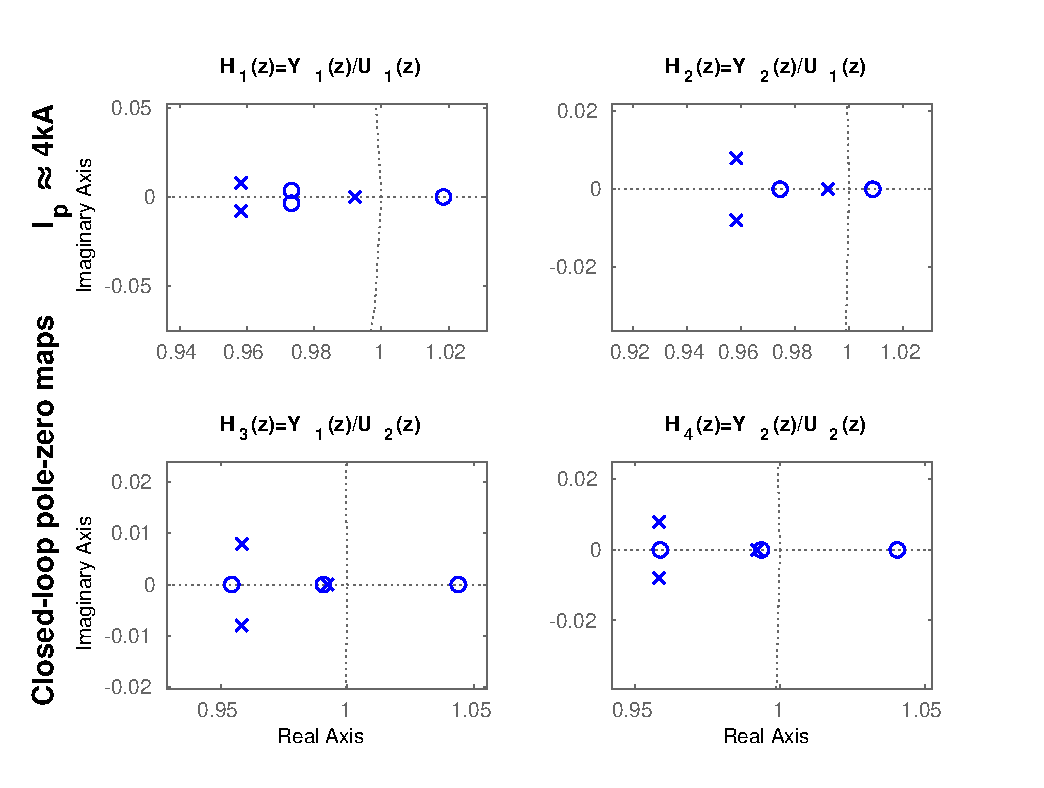
\includegraphics[width=0.85\textwidth]{Chp5/PoleZero/PoleZeroClosePosZoom.eps}
	\caption{Zoom to the stability border of the pole-zero maps in closed loop for the model when $I_p\approx 4 kA$.\label{PoleZeroClosePosZoom}}
\end{figure}
	


\begin{figure}
	\centering
	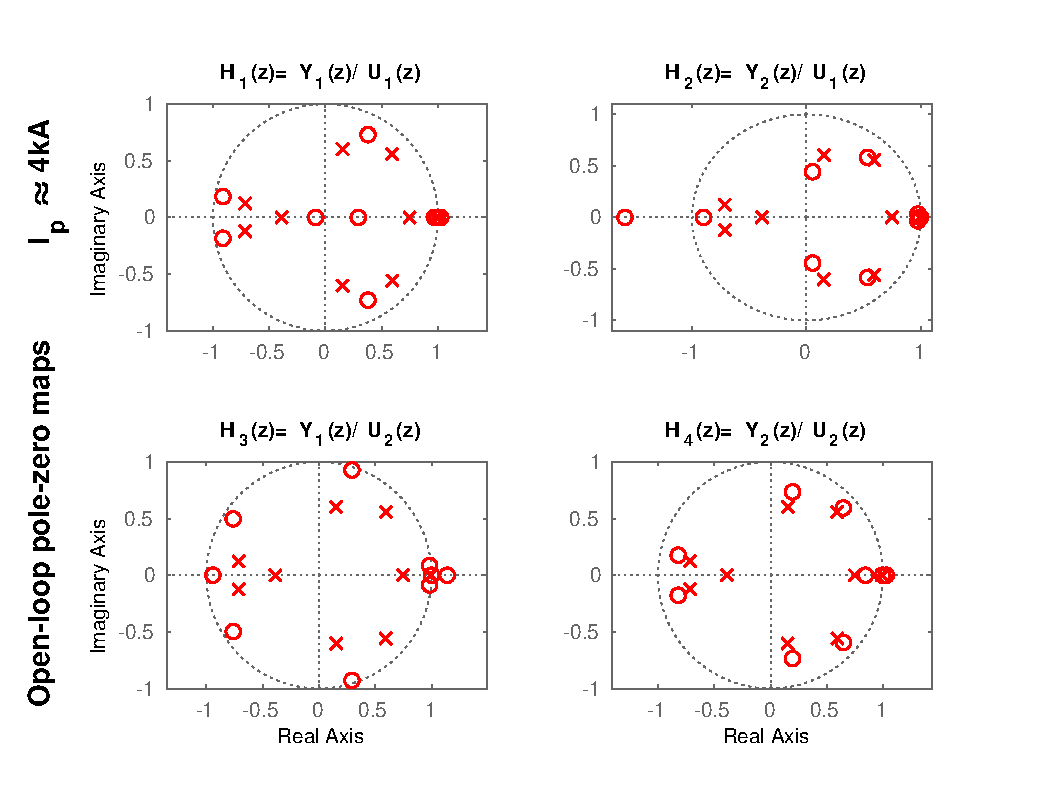
\includegraphics[width=0.85\textwidth]{Chp5/PoleZero/PoleZeroOpenPos.eps}
	\caption{  Pole-zero maps in open loop for the model when $I_p\approx 4 kA$. Superposition  of poles and zeros can be seen in the four transfer functions. \label{PoleZeroOpenPos}}
\end{figure}	

\begin{figure}
	\centering
	\includegraphics[width=0.85\textwidth]{Chp5/PoleZero/PoleZeroOpenPosZoom.eps}
	\caption{Zoom to the stability border of the pole-zero maps in open loop for the model when $I_p\approx 4 kA$. \label{PoleZeroOpenPosZoom}}
\end{figure}

%% Negatives
\begin{figure}
	\centering
	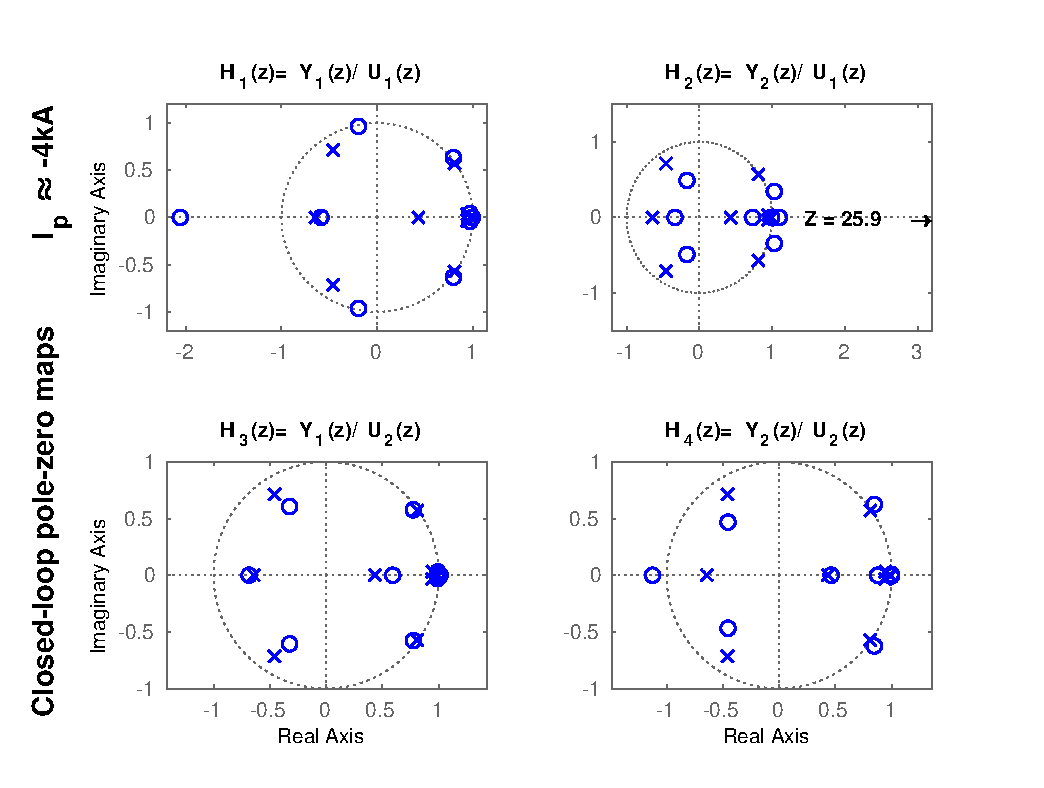
\includegraphics[width=0.85\textwidth]{Chp5/PoleZero/PoleZeroCloseNeg.eps}
	\caption{ Pole-zero maps in closed loop for the model when $I_p\approx -4 kA$. Superposition  of poles and zeros can be seen in the four transfer functions. In the transfer function $H_2(z)$ should be noticed the zero far from the unitary circumference. \label{PoleZeroCloseNeg}}
\end{figure}	

\begin{figure}
	\centering
	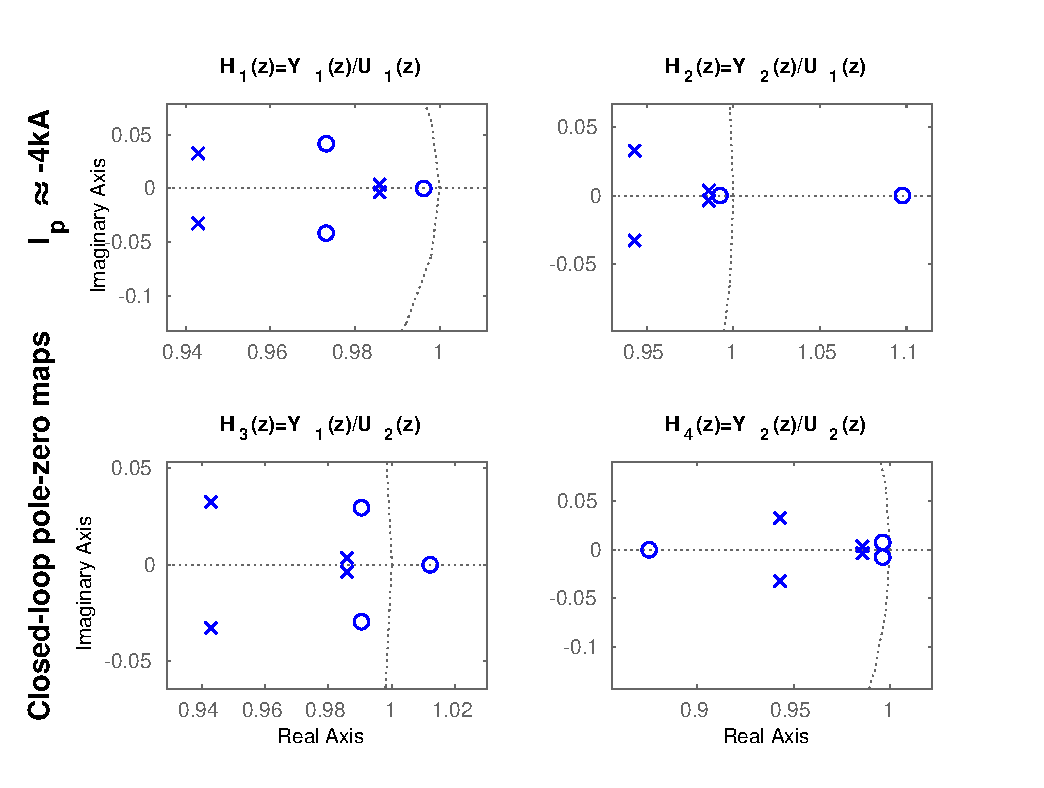
\includegraphics[width=0.85\textwidth]{Chp5/PoleZero/PoleZeroCloseNegZoom.eps}
\caption{Zoom to the stability border of the pole-zero maps in closed loop for the model when $I_p\approx -4 kA$.	\label{PoleZeroCloseNegZoom}}
\end{figure}	


\begin{figure}
	\centering
	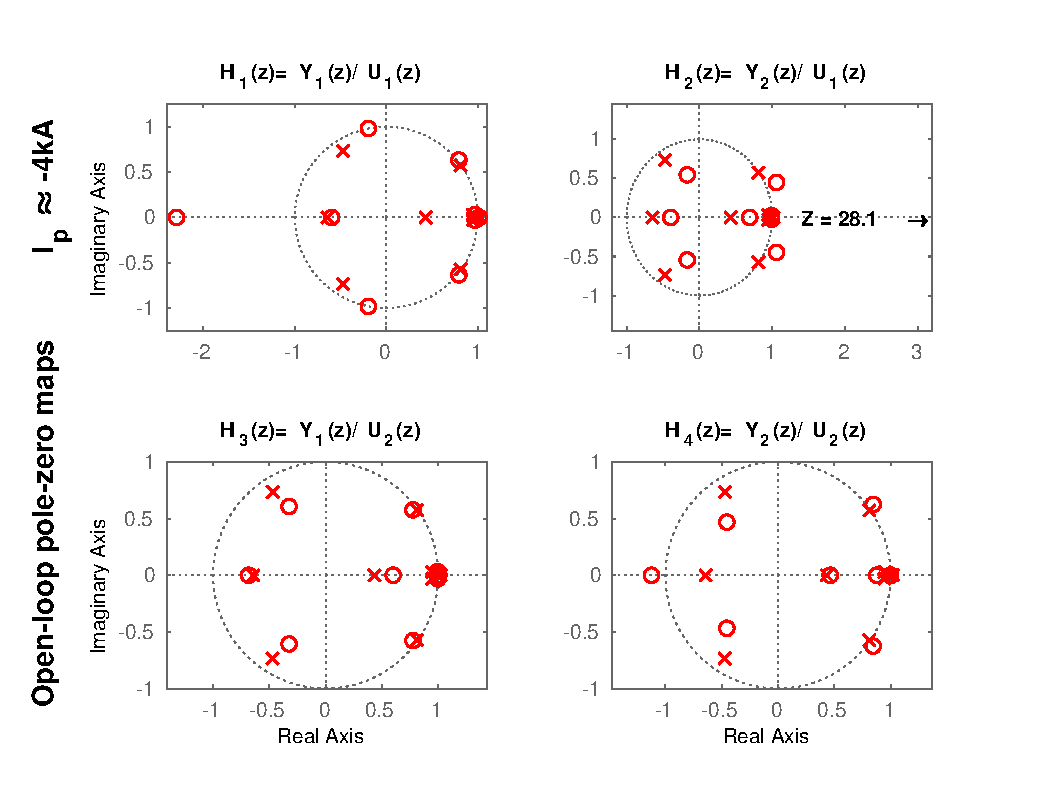
\includegraphics[width=0.85\textwidth]{Chp5/PoleZero/PoleZeroOpenNeg.eps}
	\caption{  Pole-zero maps in open loop for the model when $I_p\approx -4 kA$. Superposition  of poles and zeros can be seen in the four transfer functions. In the transfer function $H_2(z)$ should be noticed the zero far from the unitary circumference. \label{PoleZeroOpenNeg}}
\end{figure}	

\begin{figure}
	\centering
	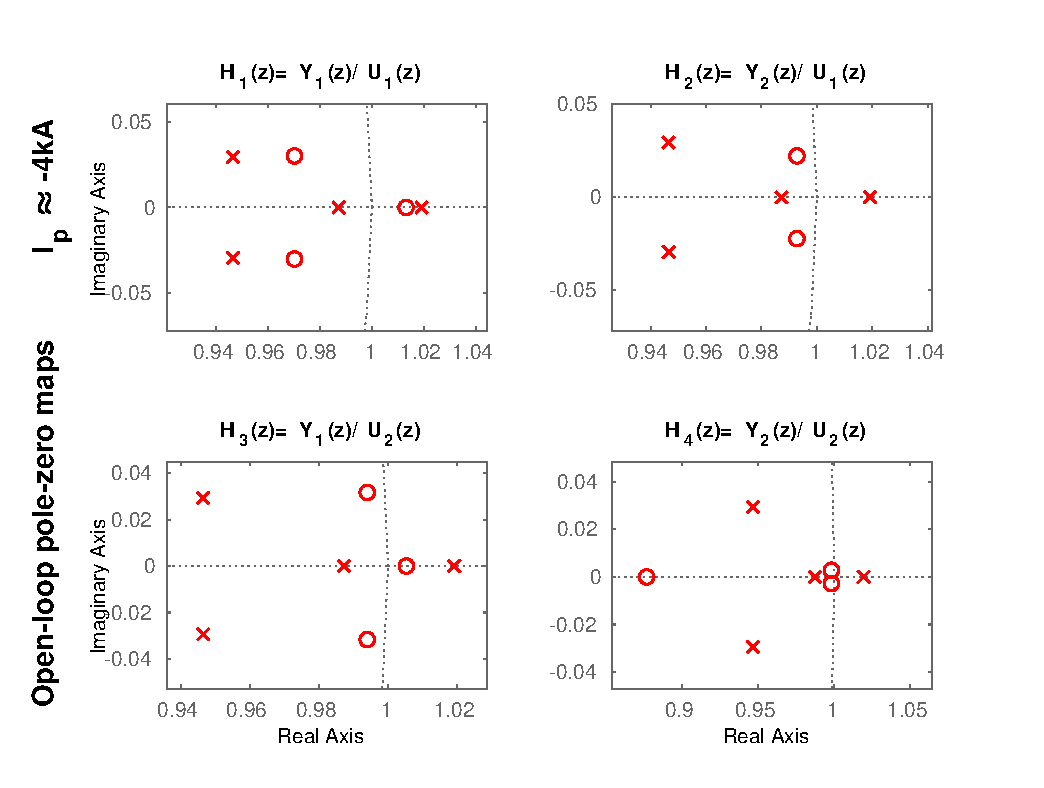
\includegraphics[width=0.85\textwidth]{Chp5/PoleZero/PoleZeroOpenNegZoom.eps}
\caption{Zoom to the stability border of the pole-zero maps in open loop for the model when $I_p\approx -4 kA$.	\label{PoleZeroOpenNegZoom}}
\end{figure}


In this plots is possible to observe several important details which allow to understand more the dynamics of the systems. Pole-zero cancellation of stables poles will not cause any serious problem in the overall system except if the canceled pole is unstable. \smallskip

$\bullet$ Positive cases
\smallskip

$\bullet$ Non-minimum phase ~\cite[Chapter~6]{Ogata2009}
\section{Plasma current centroid position control results}

This section addresses the latest results from the real-time implementation of control algorithms in ISTTOK.  

Assure a gentle transfer towards the nominal point of operation, and only if the system is in the vicinity of the desired set point, one switches from manual to automatic.

\subsection{PID control and LQR control results}

This section addresses the obtained  experimental results in ISTTOK's plasma discharges using PID and MIMO-LQR controllers for the plasma centroid position feedback. Table ~\ref{TableControl} summarizes the root-mean squared error (RMSE) for several plasma discharges for positive and negative plasma current and with different set points, the time traces for all discharges presented in the table can be found in appendix~\ref{Control_Results}.\smallskip

\begin{figure}
	\centering
	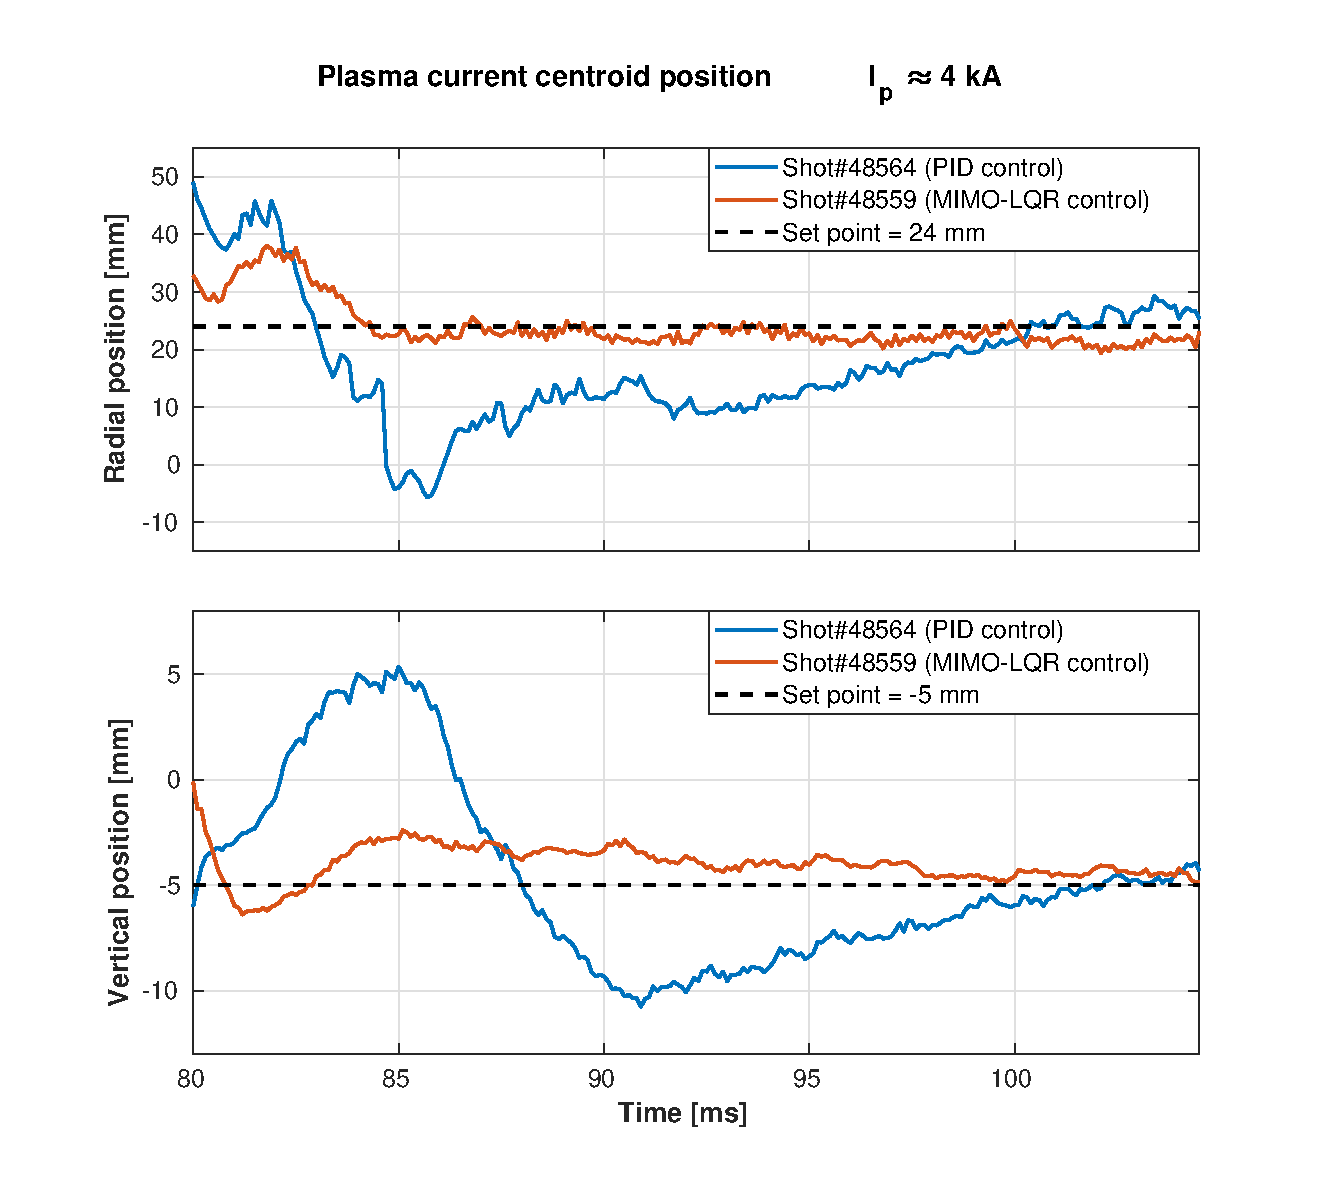
\includegraphics[width=0.8\textwidth]{Chp5/PIDvsMIMO_564_559_2.eps}
	\label{564_559}
\end{figure}

\begin{figure}
	\centering
	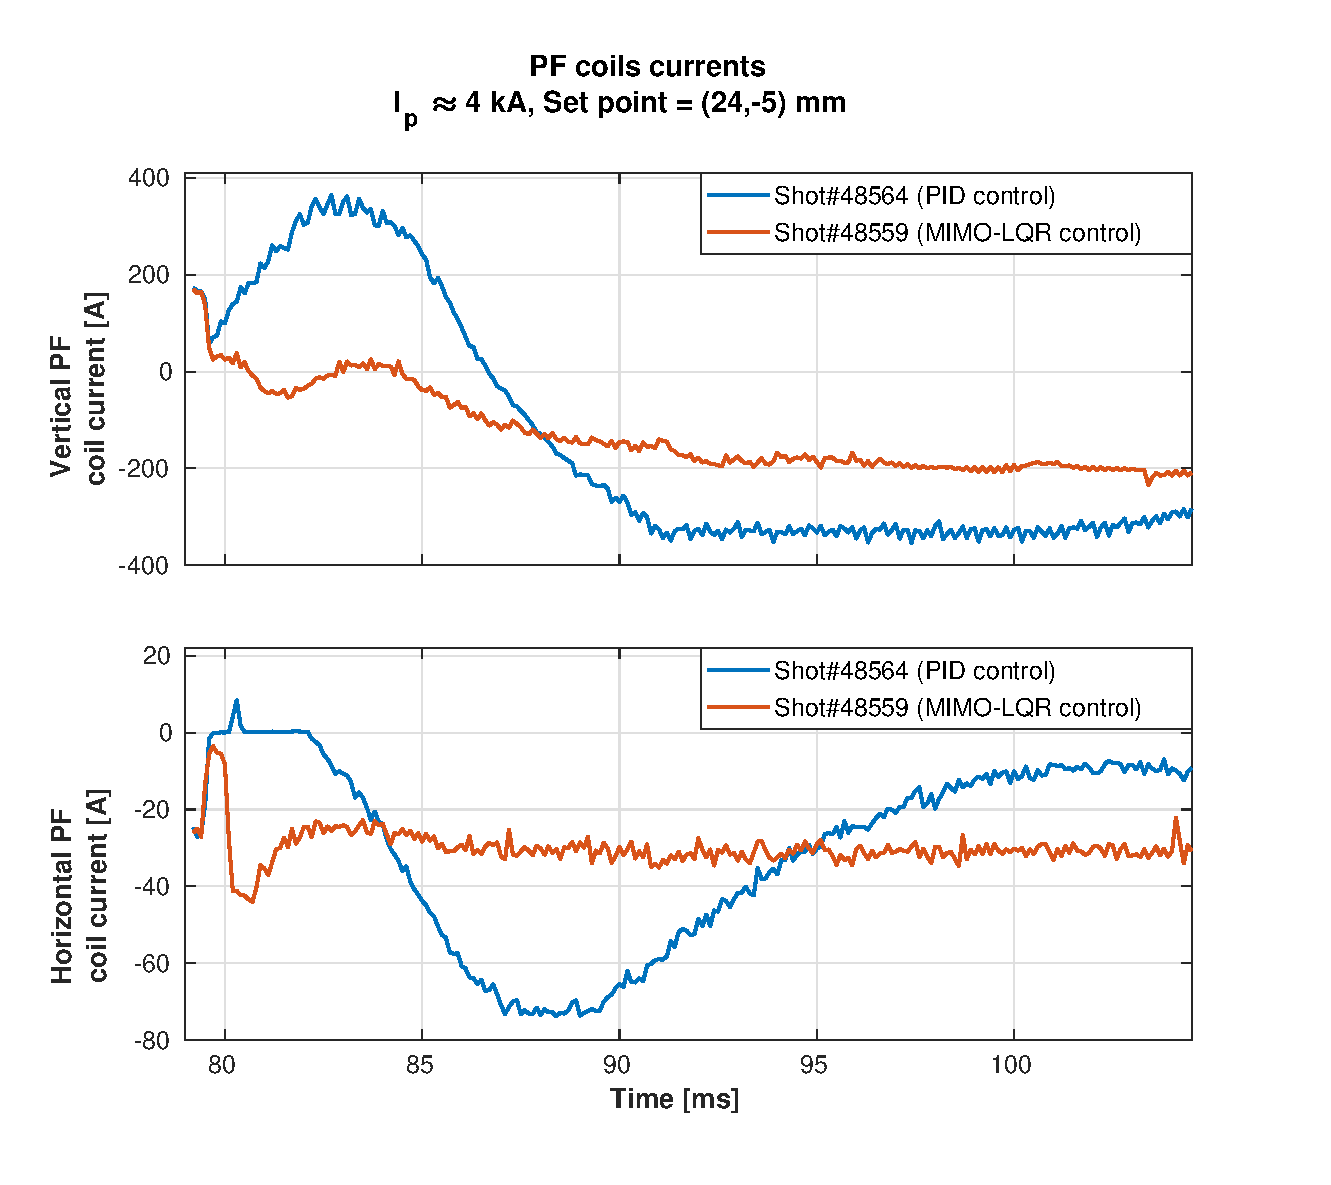
\includegraphics[width=0.8\textwidth]{Chp5/PIDvsMIMO_564_559_curr_2.eps}
	\label{564_559curr}
\end{figure}

\begin{figure}
	\centering
	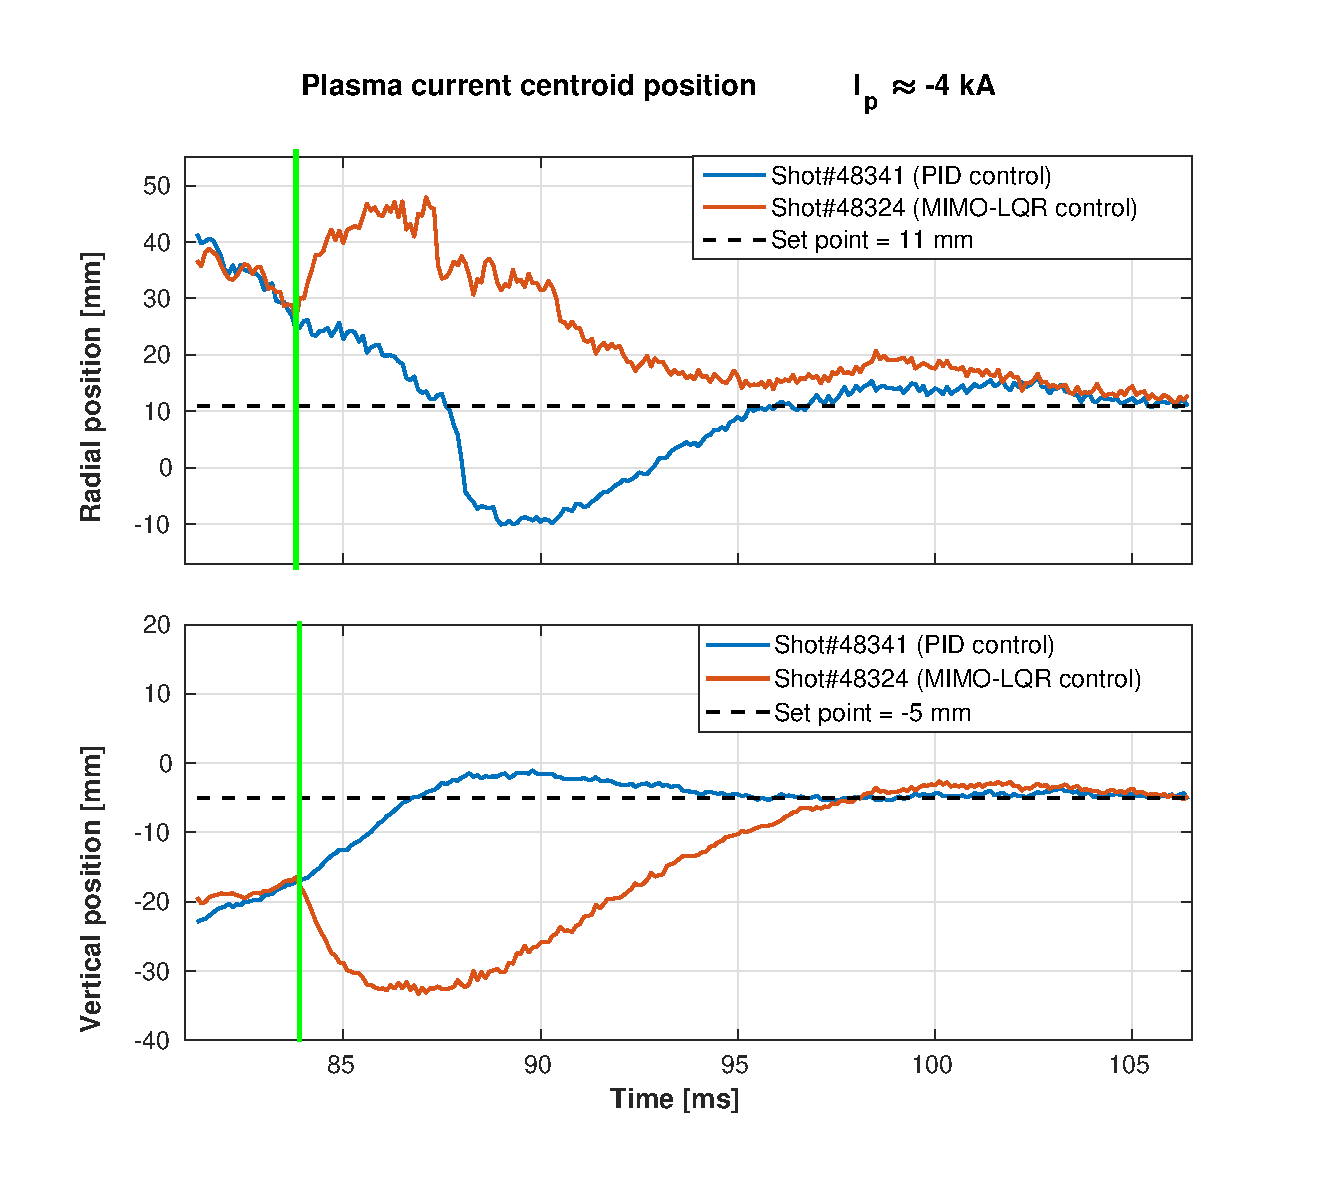
\includegraphics[width=0.8\textwidth]{Chp5/PIDvsMIMO_341_324_2.eps}
	\label{341_342}
\end{figure}

\begin{figure}
	\centering
	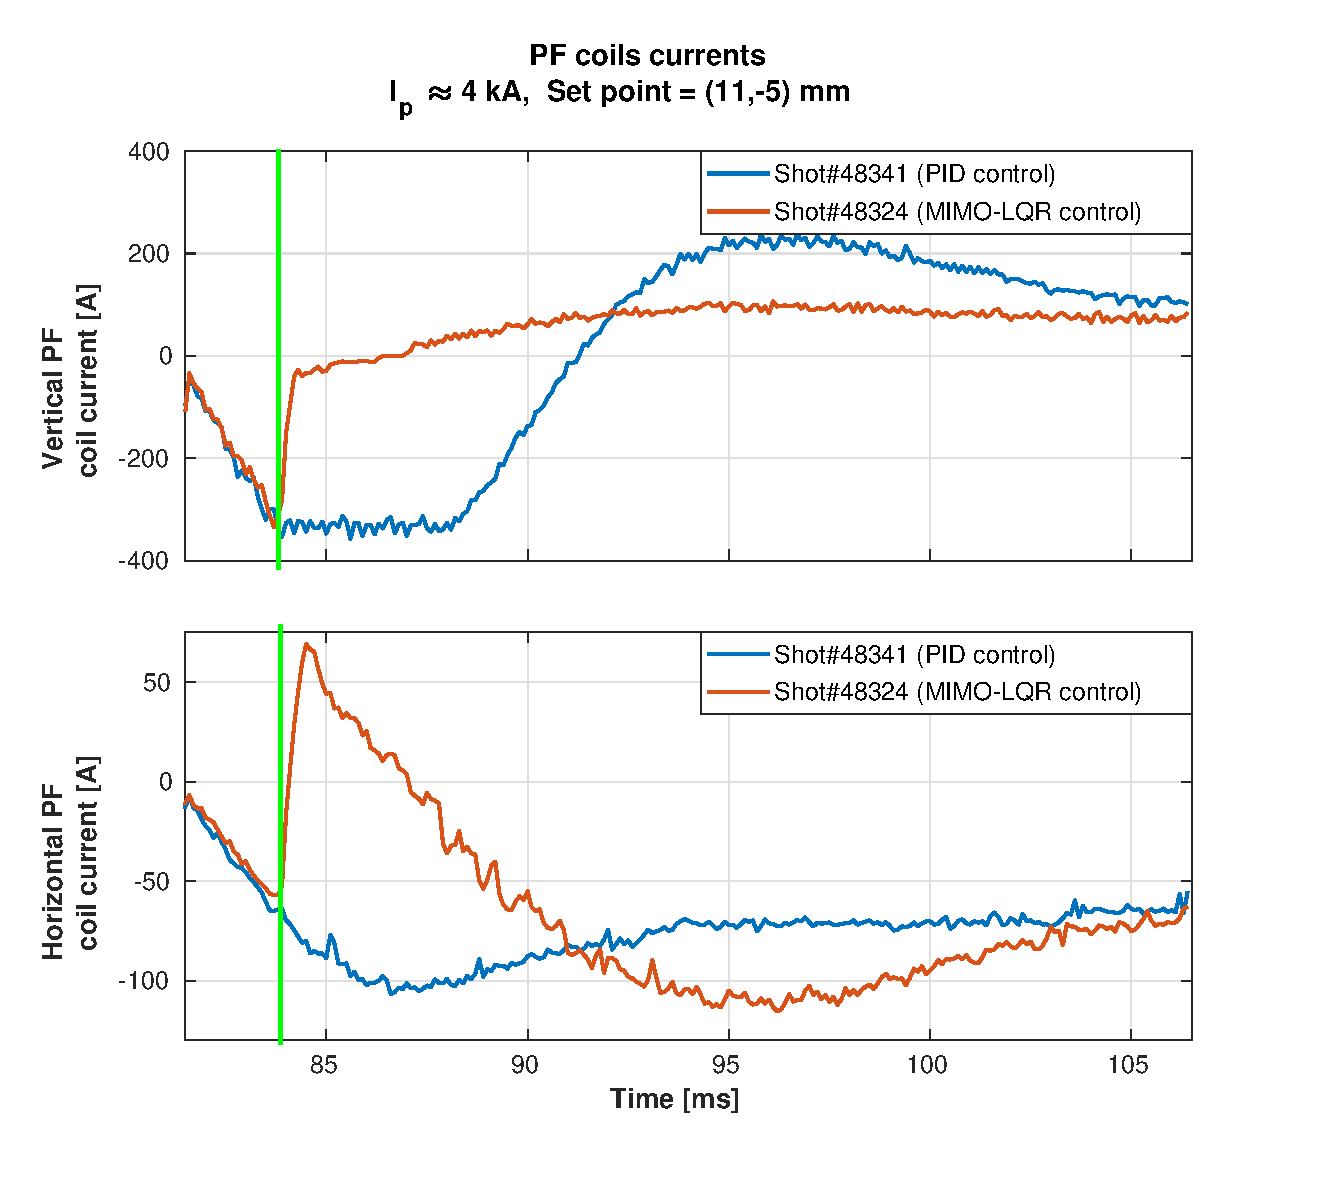
\includegraphics[width=0.8\textwidth]{Chp5/PIDvsMIMO_341_324_curr_2.eps}
	\label{341_342_curr}
\end{figure}


%
%\begin{center}
%	\begin{longtable}{||c| c| c| c|c||} 
%		\hline
%		\rowcolor{color2}
%		\textbf{Control} &  \textbf{Shot \#} &\textbf{RMSE (R,z) mm} & \textbf{ Set point (R,z) mm} &\ $\mathbf{I_p}$ \\ [0.5ex] 
%		\hline\hline
%		PID & 48564 &  (13.73, 4.4102) & (24, -5)&  $\approx 4 kA$ \\ 
%		\hline
%		MIMO LQR & 48559 & (4.2252, 1.4215 ) & (24, -5)&  $\approx 4 kA$	\\
%		\hline
%		PID & 48563 & (13.6717,	4.1652)  & (24, -4)& $\approx 4 kA$ \\ 
%		\hline
%		MIMO LQR & 48561 & (8.1047,	3.2752) & (24, -4)& $\approx 4 kA$ \\
%		\hline
%		PID & 48556 & (12.0315,	3.3217)  & (32, -5)& $\approx 4 kA$  \\ 
%		\hline
%		MIMO LQR & 48555 & (4.2618, 2.4698) & (32, -5) &  $\approx 4 kA$ \\
%		\hline
%		PID & 48551 & (13.9998,	3.3431)  & (27, -5) &  $\approx 4 kA$ \\ 
%		\hline
%		MIMO LQR & 48554 & (5.9830, 2.0062)  & (27, -5) &  $\approx 4 kA$ \\
%		\hline
%		PID & 48515 & (6.0178,	2.6123)  & (30, -5) & $\approx 4 kA$ \\ 
%		\hline
%		MIMO LQR & 48541 & (5.8372,	1.7664) & (30, -5) &  $\approx 4 kA$\\
%		\hline
%		PID & 48544 & (4.8745,	2.5167)  & (32, -4)& $\approx 4 kA$ \\ 
%		\hline
%		MIMO LQR & 48542 & (4.4346,	3.6573) & (32, -4)&  $\approx 4 kA$ \\
%		\hline
%		PID & 48546 & (11.4560, 3.4765)  & (27, -7)&   $\approx 4 kA$\\ 
%		\hline
%		MIMO LQR & 48548 & (7.6745, 4.1569) & (27, -7)&  $\approx 4 kA$ \\
%		\hline
%		PID & 48341 & (12.0959,	5.7652)  & (11, -5)& $\approx -4 kA$\\ 
%		\hline
%		MIMO LQR & 48324 &  (15.4768,	14.3436)& (11, -5)& $\approx -4 kA$ \\
%		\hline
%		PID & 48340 & ( 11.7701, 5.9599) & (11.2, -5.5)&  $\approx -4 kA$\\ 
%		\hline
%		MIMO LQR & 48338 & (11.5260,	12.6226) & (11.2, -5.5) &  $\approx -4 kA$\\
%		\hline
%		PID & 48343 &(15.7675,	5.7453)   & (12, -5)&  $\approx -4 kA$  \\ 
%		\hline
%		MIMO LQR & 48342 & (14.5168,	14.4329) & (12, -5)&  $\approx -4 kA$  \\
%		\hline
%		PID & 48346 & (12.4228,	6.1541)  & (12.2, -5.3)& $\approx -4 kA$\\ 
%		\hline
%		MIMO LQR & 48345 & (9.7513,	13.0338) & (12.2, -5.3)& $\approx -4 kA$ \\
%		\hline
%		PID & 48349 & (19.3397,	5.5406)  & (11.5, -5.6)&$\approx -4 kA$  \\ 
%		\hline
%		MIMO LQR & 48348 & (9.1727,	13.1505) & (11.5, -5.6)&$\approx -4 kA$  \\
%		\hline
%		PID & 48352 &  (15.2181,	6.5395) & (10.8, -4.7) &$\approx -4 kA$ \\ 
%		\hline
%		MIMO LQR & 48354 & (14.6405,	13.7307) & (10.8, -4.7)& $\approx -4 kA$ \\
%		\hline
%		PID & 48351 &  (13.4078, 5.8769) & (13.2, -5.6)& $\approx -4 kA$ \\ 
%		\hline
%		MIMO LQR & 48350 & (13.9320,	14.4940) & (13.2, -5.6)&$\approx -4 kA$  \\[1ex]
%		\hline
%		\caption{Centroid position RMSE comparison between PID and MIMO-LQR controlled discharges for different set points and plasma current scenarios.}
%	\end{longtable}
%\label{TableControl}
%
%\end{center}

\begin{center}
	\begin{longtable}{||c| c| c| c|c||} 
		\hline
		\rowcolor{color2}
		\textbf{Control} &  \textbf{Shot \#} &\textbf{RMSE (R,z) mm} & \textbf{ Set point (R,z) mm} &\ $\mathbf{I_p}$ \\ [0.5ex] 
		\hline\hline
		PID & 48564 &  (13.73, 4.4102) & \multirow{ 2}{*}{(24, -5)}&  $\approx 4 kA$ \\ 
		\cline{1-3} \cline{5-5}
		MIMO LQR & 48559 & (4.2252, 1.4215 ) & &  $\approx 4 kA$	\\
		\hline
		PID & 48563 & (13.6717,	4.1652)  & \multirow{ 2}{*}{(24, -4)}& $\approx 4 kA$ \\ 
		\cline{1-3} \cline{5-5}
		MIMO LQR & 48561 & (8.1047,	3.2752) & & $\approx 4 kA$ \\
		\hline
		PID & 48556 & (12.0315,	3.3217)  & \multirow{ 2}{*}{(32, -5)}& $\approx 4 kA$  \\ 
		\cline{1-3} \cline{5-5}
		MIMO LQR & 48555 & (4.2618, 2.4698) &  &  $\approx 4 kA$ \\
		\hline
		PID & 48551 & (13.9998,	3.3431)  & \multirow{ 2}{*}{(27, -5)} &  $\approx 4 kA$ \\ 
		\cline{1-3} \cline{5-5}
		MIMO LQR & 48554 & (5.9830, 2.0062)  &  &  $\approx 4 kA$ \\
		\hline
		PID & 48515 & (6.0178,	2.6123)  & \multirow{ 2}{*}{(30, -5)} & $\approx 4 kA$ \\ 
		\cline{1-3} \cline{5-5}
		MIMO LQR & 48541 & (5.8372,	1.7664) &  &  $\approx 4 kA$\\
		\hline
		PID & 48544 & (4.8745,	2.5167)  & \multirow{ 2}{*}{(32, -4)}& $\approx 4 kA$ \\ 
		\cline{1-3} \cline{5-5}
		MIMO LQR & 48542 & (4.4346,	3.6573) & &  $\approx 4 kA$ \\
		\hline
		PID & 48546 & (11.4560, 3.4765)  & \multirow{ 2}{*}{(27, -7)}&   $\approx 4 kA$\\ 
		\cline{1-3} \cline{5-5}
		MIMO LQR & 48548 & (7.6745, 4.1569) & &  $\approx 4 kA$ \\
		\hline
		PID & 48341 & (12.0959,	5.7652)  & \multirow{ 2}{*}{(11, -5)}& $\approx -4 kA$\\ 
		\cline{1-3} \cline{5-5}
		MIMO LQR & 48324 &  (15.4768,	14.3436)& & $\approx -4 kA$ \\
		\hline
		PID & 48340 & ( 11.7701, 5.9599) & \multirow{ 2}{*}{(11.2, -5.5)}&  $\approx -4 kA$\\ 
		\cline{1-3} \cline{5-5}
		MIMO LQR & 48338 & (11.5260,	12.6226) &  &  $\approx -4 kA$\\
		\hline
		PID & 48343 &(15.7675,	5.7453)   & \multirow{ 2}{*}{(12, -5)}&  $\approx -4 kA$  \\ 
		\cline{1-3} \cline{5-5}
		MIMO LQR & 48342 & (14.5168,	14.4329) & &  $\approx -4 kA$  \\
		\hline
		PID & 48346 & (12.4228,	6.1541)  & \multirow{ 2}{*}{(12.2, -5.3)}& $\approx -4 kA$\\ 
		\cline{1-3} \cline{5-5}
		MIMO LQR & 48345 & (9.7513,	13.0338) & & $\approx -4 kA$ \\
		\hline
		PID & 48349 & (19.3397,	5.5406)  & \multirow{ 2}{*}{(11.5, -5.6)}&$\approx -4 kA$  \\ 
		\cline{1-3} \cline{5-5}
		MIMO LQR & 48348 & (9.1727,	13.1505) & &$\approx -4 kA$  \\
		\hline
		PID & 48352 &  (15.2181,	6.5395) & \multirow{ 2}{*}{(10.8, -4.7)} &$\approx -4 kA$ \\ 
		\cline{1-3} \cline{5-5}
		MIMO LQR & 48354 & (14.6405,	13.7307) & & $\approx -4 kA$ \\
		\hline
		PID & 48351 &  (13.4078, 5.8769) & \multirow{ 2}{*}{(13.2, -5.6)}& $\approx -4 kA$ \\ 
		\cline{1-3} \cline{5-5} 
		MIMO LQR & 48350 & (13.9320,	14.4940) & &$\approx -4 kA$  \\
		\hline 
		\caption{Centroid position RMSE comparison between PID and MIMO-LQR controlled discharges for different set points and plasma current scenarios.}
	\end{longtable}
	\label{TableControl}
	
\end{center}

